%
% File: chap01.tex
% Author: Victor F. Brena-Medina
% Description: Introduction chapter where the biology goes.
%
\let\textcircled=\pgftextcircled
\chapter{Introduction}
\label{chap:intro}

\initial{T}he technique of automatic video content analysis (VCA) is one of the most important areas of Computer Vision and Artificial Intelligence. With this technique, machines are able to recognize objects, human activities and events in videos.   Thus, it can be widely used in many domains, such as human-computer interaction, video classification, entertainment, self-driving, public safety and security, home automation, etc. Action and interaction analysis is one of the most common uses of VCA which focuses on the analysis of human activities, such as the  recognition/detection of the action of a single person or recognition/detection of the interaction of two or more people.


%=======
\section{Background}
\label{sec:intro_sec01}
When we talk about human action, we usually mean the activity of a single person. But in truth, human interaction is more complex and generally contains three cases: human-human interaction between two or more people, such as hand-shaking; human-object-human interaction like a person passing an object to another person; and human-object interaction like a person pushing a table.
\par 
The goal of \textbf{human action/interaction recognition} in videos is to determine the action/interaction labels. And the goal of \textbf{human action/interaction detection} in a video is to locate a specific action/interaction spatially and temporally in the video. 
\par 
Although a lot of excellent methods and datasets have been published in the last decade in the area of action recognition, it is still a challenging task and is far from being solved. Comparatively, the related work in the domain of interaction recognition and detection is relatively scarce. This is because the job of interaction recognition and detection is even more challenging than that of action recognition and detection.  
 
\par
The main challenges of action and interaction recognition and detections in real scenes mainly include: 
\begin{enumerate}
	\item Various camera views. The videos which will be analysed could be taken from different viewpoints which may have never been seen before in the training data. For example, Figure \ref{fig:challenges} (a) illustrates four videos of the same biking little girl being filmed from four different camera views. The features extracted from these videos can be different, which would then make it hard for the classifier to learn to discriminate them as the same activity. 
	\item Complex background. The background of the action/interaction could vary and even be totally different. For example, Figure \ref{fig:challenges} (b) illustrates four diving videos taken with totally different backgrounds with large camera motions. For those feature descriptors that extract features from not only the segmented person but also from the background. Then the features extracted from the background would largely confuse the classification results.  
	\item Usually, a single action video clip contains at least hundreds of frames. Therefore, there might exist many irrelevant frames which would, in turn, confuse the analysis process. For instance, a video clip of a basketball game may contain frames of commentators and the audiences which wouldn't be relevant. 
	\item It is hard to get decent performance on a small training set. But sometimes we only have small scale target datasets with very limited training samples. Such situation is even worse for the task of interaction video analysis since the related dataset is scarce compared with the action video analysis.
	\item Compared with action video analysis, extra features like relative position and orientation between the people involved in the interaction need to be taken into consideration, which makes the representation of features more complex. 
\end{enumerate}

\begin{figure}
	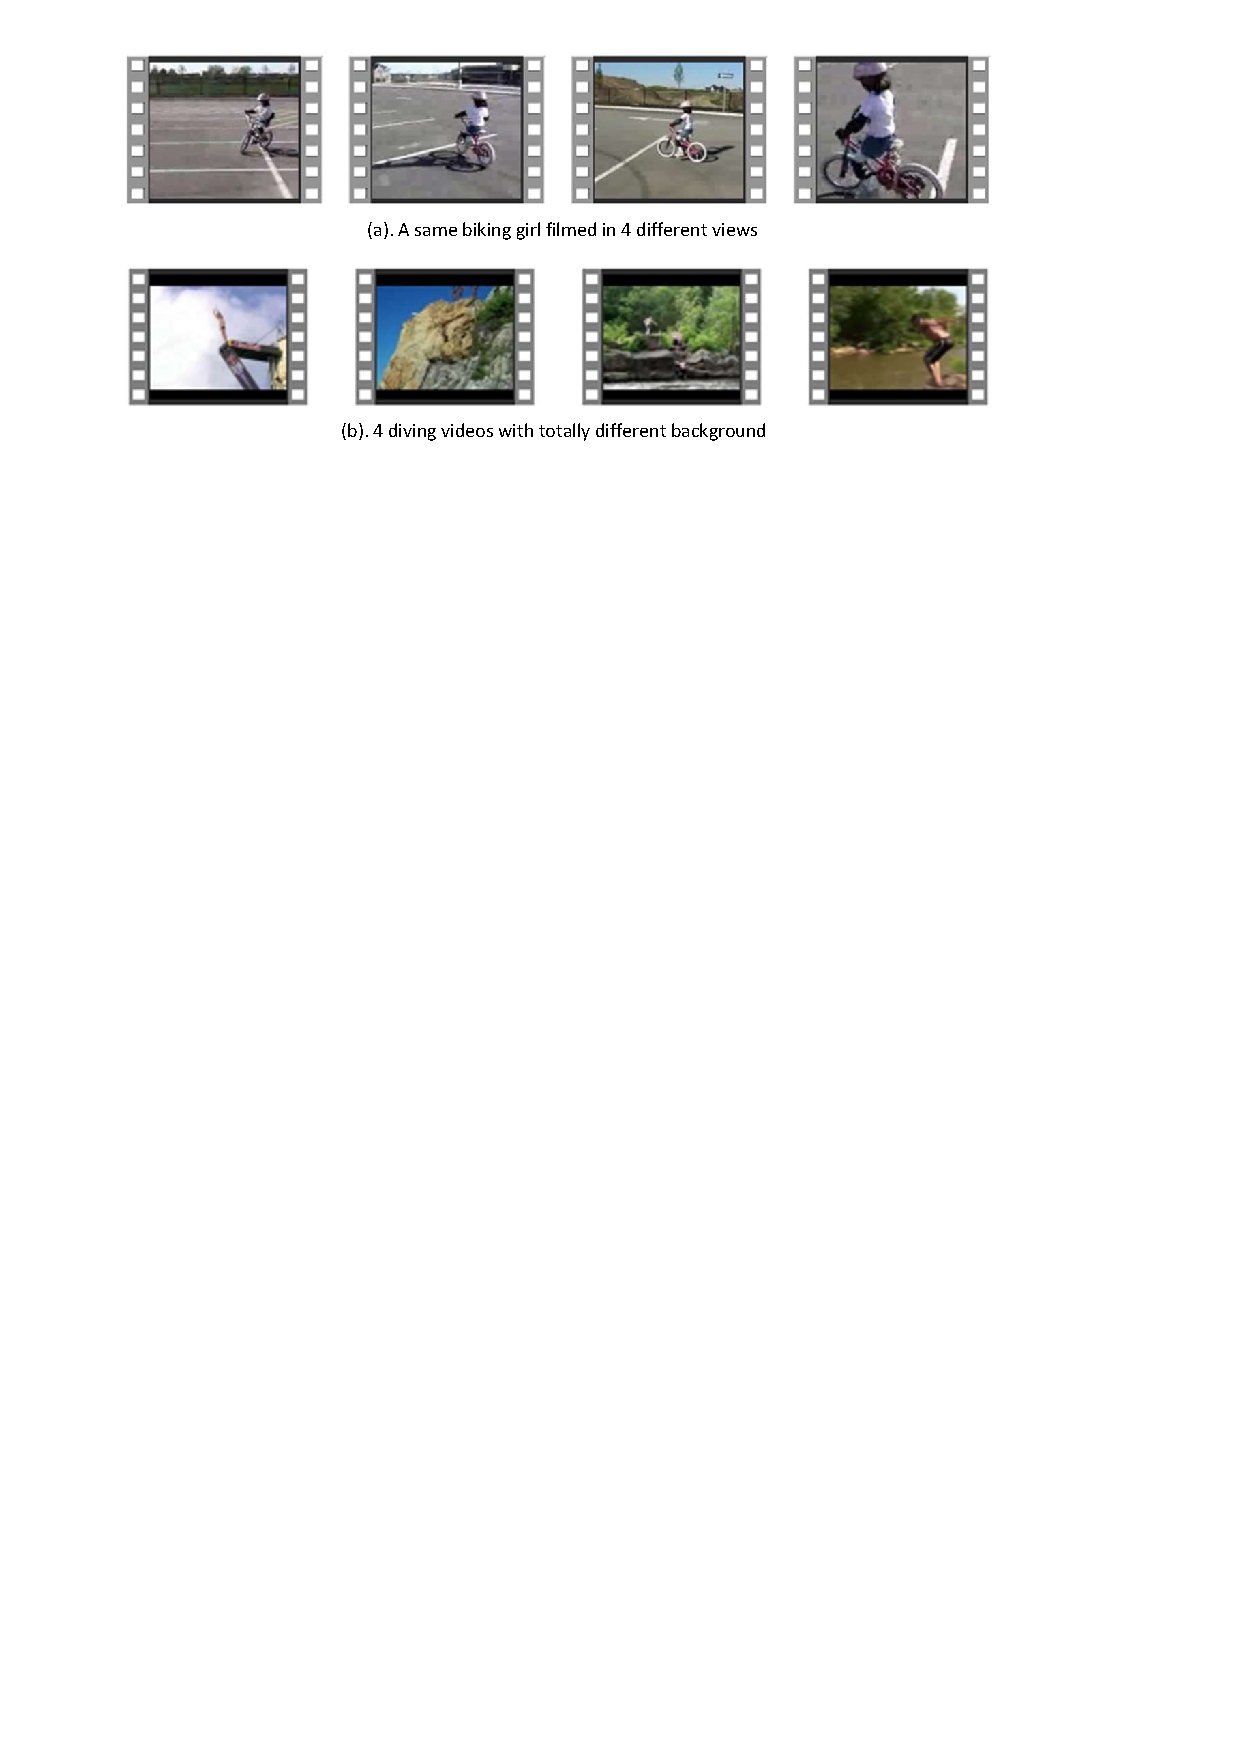
\includegraphics[trim=2cm 22cm 0cm 1cm]{fig01/challenges.pdf}
	\caption{Illustration of some challenges of video analysis. }
	\label{fig:challenges}
\end{figure}

Some of the related works for interaction analysis are \cite{patron2010}, \cite{Gemeren2015}, \cite{narayan2014} and \cite{choi2012}. The works of Patron-Perez et al. \cite{patron2010} and  Gemeren et al. \cite{Gemeren2015} focus on the relative information between the people involved in the interaction, such as their relative position and orientation in relevant body parts and, then uses hand-crafted feature descriptors, such as histograms of orientated gradients (HOG \cite{hog}) and histograms of optical flow (HOF \cite{hof}), to describe those interaction features. The work of Narayan et al. \cite{narayan2014} combines the improved trajectory features and the foreground motion map features to describe interaction features. In contrast, Choi et al. \cite{choi2012} introduce a hierarchical method, which first detects and tracks the location of each person and then learns to analyse the atomic action of each person. Lastly, it uses the atomic action to infer the collective interaction label. The atomic action is also represented by the hand-crafted feature descriptors, such as HOG and bag of video words (BoV \cite{bov}).
\par 
In this thesis project, we adopt a similar hierarchical architecture with the work of Choi et al. with two main changes: 1). we use the deep learning feature descriptors to represent the atomic action for each person involved in the interaction instead of hand-crafted feature descriptors; 2). Besides having the networks learning atomic features of each person, we add  an additional deep learning network to learn the features of relative position and orientation.   

\section{Project Goals}
\label{sec:intro_sec02}

In this thesis project, we focus on the recognition and detection of two-person interaction. The goals of this thesis project include: 
\begin{enumerate}
	\item To do interaction recognition based on the target dataset. The inputs are the segmented specific interaction videos and the outputs are the predicted class labels.
	\item To do interaction detection based on the target dataset. The input is the un-segmented videos and the output is the spatial and temporal location of specified classes. 
	\item Construct a hierarchical multi-level network to learn the features of interaction. Hierarchical network means that we first learn atomic action features for each person involved in interaction, then combine these features to learn interaction features. Multi-level network means that we have a global first level network which learns global interaction features, such as the relative position and orientation between the people involved in the interaction and a second level network which learns the atomic actions of each person.
\end{enumerate}

\section{Contributions}
\label{sec:intro_sec03}

We mainly have the following contributions for the interaction video analysis: 
\begin{enumerate}
	\item We introduce deep learning feature descriptors that address the interaction recognition and detection with only a small scale target interaction video dataset available. 
	\item We introduce a hierarchical multi-level framework that will be used for interaction video analysis tasks.
	\item We introduce a two-step method for interaction detection in videos.
\end{enumerate}

\section{Outline}
\label{sec:intro_outline}
In the next chapter, we will introduce action and interaction video analysis related works including various methodologies and related datasets. In Chapter 3 and Chapter 4, we will describe our overall architecture and low-level design of this project in detail. In Chapter 5, we will introduce the experiments designs, their experimental results, and analyse them. At last, we will give the conclusions and possible future works of this project.
%=========================================================